\begin{flushleft}
Abbiamo notato che i due metodi (in particolar modo la forma di Simpson) senza una condizione aggiuntiva rispetto a quella dell'errore è possibile che ciclino all'infinito. Inseriamo così un numero massimo di iterazioni della ricorsione negli argomenti della funzione:
\lstinputlisting[language=Matlab]{cap_5/trapeziAdattiva.m}
\lstinputlisting[language=Matlab]{cap_5/simpsonAdattiva.m}
Con questi 2 metodi è possibile creare lo script di risoluzione seguente:
\lstinputlisting[language=Matlab]{cap_5/es3/es3.m}
Gli output che restituisce sono i seguenti:
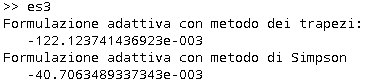
\includegraphics[left, width=300px, height=100px]{cap_5/es3/es53.png}
\end{flushleft}